
\section{Pengembangan Prototipe \textit{High-Fidelity} Iterasi 1}
\label{sec:hifi_1}

Prototipe \textit{high-fidelity} adalah implementasi dari solusi desain yang dibuat sedekat mungkin dengan produk aslinya. Prototipe \textit{high-fidelity} memiliki fungsionalitas, elemen visual, dan interaksi yang lebih lengkap daripada prototipe \textit{low-fidelity}. \parencite{PreeceRogersSharp15} Prototipe yang dirancang mengembangkan seluruh tampilan pada Tabel \ref{tab:daftar_lofi_halaman} dan Tabel \ref{tab:daftar_lofi_widget} di bagian \ref{sec:lofi} pengembangan prototipe \textit{low-fidelity}, serta menerapkan lebih banyak prinsip desain sesuai yang telah disebutkan pada bagian \ref{tab:prinsip_desain}. Tujuan dari perancangan prototipe \textit{high-fidelity} ini adalah untuk mencapai \textit{usability goals} dan \textit{user experience goals} yang telah diharapkan dari analisis pada bagian \ref{subsec:analisis_goals}. Sebelum membuat prototipe, perlu ditentukan batasan implementasi, aspek antarmuka pengguna, serta komponen desain.


\subsection{Aspek Antarmuka Pengguna}
\label{subsec:antarmuka}

Secara umum, aspek-aspek antarmuka yang digunakan pada prototipe \textit{high-fidelity} ini mengacu pada sistem desain Material Design yang dibuat oleh Google. Panduan lengkap tentang Material Design dapat dilihat pada websitenya (\href{https://material.io/design}{https://material.io/design}). Material Design dipilih karena prototipe \textit{high-fidelity} ini merupakan perbaikan yang dilakukan untuk aplikasi Digital Wellbeing yang dibuat oleh Google. Aspek-aspek yang dipilih dari Material Design juga melihat aspek-aspek antarmuka dari aplikasi Digital Wellbeing awal. Berikut adalah penjelasan-penjelasan untuk setiap aspek antarmuka pada prototipe \textit{high-fidelity}  

\subsubsection{Warna}
\label{subsubsec:aspek_warna}
Warna yang digunakan dalam prototipe terbagi menjadi 3 kategori, yaitu warna primer, warna sekunder, dan warna tersier

\subsubsection{Tipografi}
\label{subsubsec:aspek_tipografi}
\textit{Typeface} yang digunakan dalam prototipe adalah Roboto, sesuai dengan \textit{typeface} yang digunakan oleh aplikasi Digital Wellbeing, dan merupakan \textit{typeface} standar yang digunakan dalam \textit{smartphone} berbasis Android.

\begin{figure}[h]
  \centering
  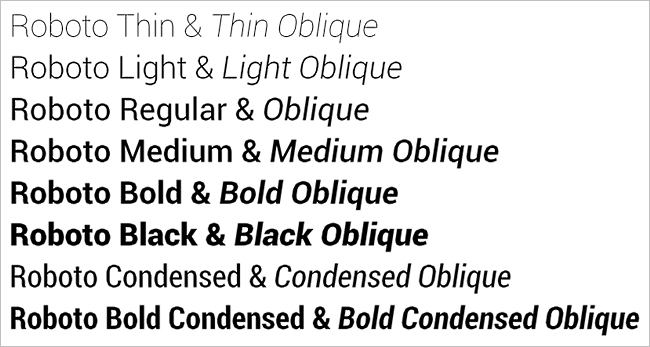
\includegraphics[width=0.6\textwidth]{chapter-4-roboto.jpg}
  \caption{\textit{Typeface} Roboto}
  \label{img:typeface}
\end{figure}

\subsubsection{\textit{Icon}}
\label{subsubsec:aspek_icon}
Icon
 
\subsubsection{Komponen Desain}
\label{subsubsec:komponen_hifi_1}

Komponen desain


\subsection{Batasan Pengembangan}
\label{subsec:batasan_hifi_1}

Pengembangan prototipe \textit{high-fidelity} ini memiliki beberapa batasan agar pengembangan dapat fokus pada tujuan pengujian. Batasan-batasan pengembangan prototipe \textit{high-fidelity} adalah sebagai berikut

\begin{enumerate}
  \item Pengembangan prototipe \textit{high-fidelity} akan menggunakan \textit{prototyping tool} Figma.
  \item Data yang digunakan dalam prototipe berupa \textit{mock data} yang ditentukan oleh desainer.
  \item Prototipe dikembangkan untuk \textit{smartphone} berdimensi layar ukuran 360x800 pixel.
  \item Prototipe tidak mendukung kemampuan untuk input data kustom, bila komponen prototipe ditujukan untuk input data maka data yang ditunjukkan telah ditentukan oleh desainer.
  \item Tampilan prototipe menggunakan Bahasa Inggris. 
  \item Fitur rekomendasi pada prototipe tidak menggunakan rekomendasi nyata atas analisis data pengguna.
  \item Homescreen pada prototipe tidak mengacu pada tampilan \textit{smartphone} merk tertentu dengan alasan fokus pada tujuan untuk menguji komponen-komponen prototipe yang tidak dapat diakses dari dalam aplikasi.
\end{enumerate}

\subsection{Implementasi Prototipe \textit{High-Fidelity}}

Implementasi Prototipe \textit{High-Fidelity}

